%----------------------------------------------------------------------------------------
%	PACKAGES AND DOCUMENT CONFIGURATIONS
%----------------------------------------------------------------------------------------

\documentclass[11pt]{article}

\usepackage{hyperref}
\usepackage{caption}
\usepackage{xcolor}
\usepackage{graphicx} % Required for the inclusion of images
\usepackage{amsmath} % Required for some math elements 
\usepackage[margin=16mm]{geometry}
\usepackage{courier}
\usepackage{listings}
\usepackage{graphicx}
\usepackage{subcaption}

\lstset{basicstyle=\footnotesize\ttfamily,breaklines=true}
\captionsetup[figure]{font=small}

\addtolength{\topmargin}{-8mm}
\addtolength{\textheight}{16mm}


\setlength\parindent{0pt} % Removes all indentation from paragraphs
\renewcommand{\labelenumi}{\alph{enumi}.} % Make numbering in the enumerate environment by letter rather than number (e.g. section 6)

%----------------------------------------------------------------------------------------
%	DOCUMENT INFORMATION
%----------------------------------------------------------------------------------------

\title{ECEN 220 \\ Lab Report 3 \\ Signals and LTI Systems}
\author{Daniel Eisen \\ 300447549}
\date{\today}

\begin{document}
\maketitle
%----------------------------------------------------------------------------------------
%	SECTION 1
%----------------------------------------------------------------------------------------
\section{Cosine FS}
\begin{figure}[h]
\begin{center}
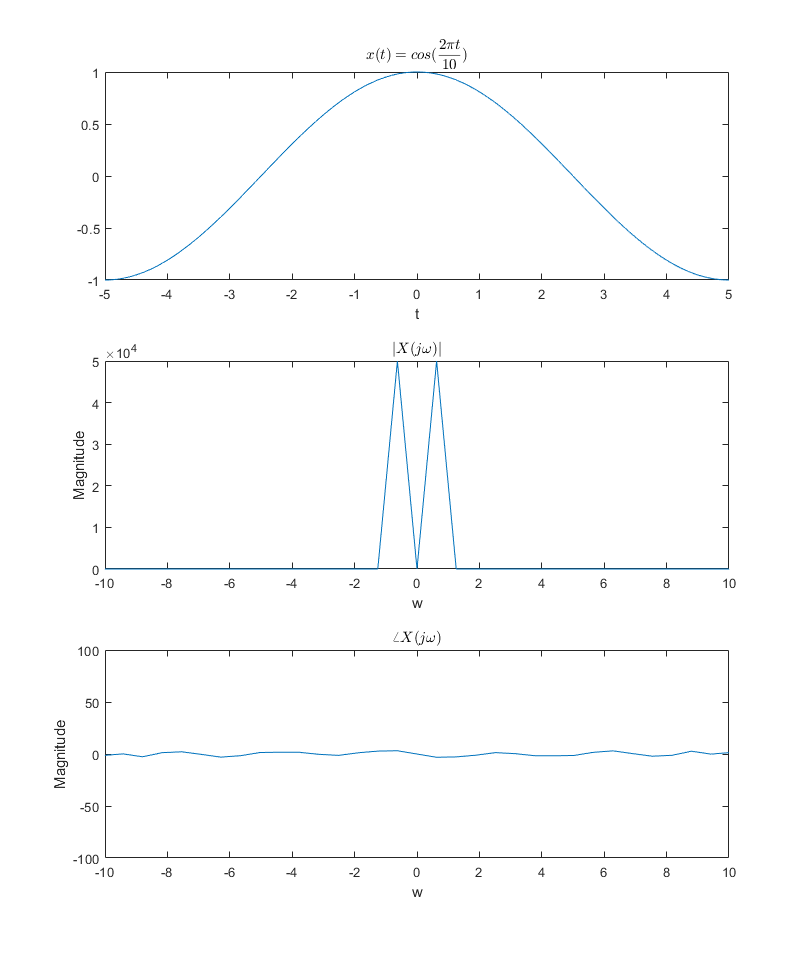
\includegraphics[width=0.5\textwidth]{q1}
\caption{(1.a) \& (1.b) Signal and Mag/Phase plots of $cos(\dfrac{2{\pi}t}{10})$}
\end{center}
\end{figure}
\paragraph*{1.c)}
The plotted magnitudes in the frequency domain are as expected, with 2 deltas at the positive and negative natural frequency of the cosine. However, due to limit of machine precision and floating point errors around zero, the phase plotting is inaccurate. Ie should be a flat zero for all $\omega$
\paragraph*{1.d)}
As the t resolution increases this doesn't effect the mag plotting due to the fact that it is just 2 deltas and those delta sample value do not change.
But as $\omega$ space is a transformed t space it to increases in resolution,
The 'discreteness' of the transforms increases. Ie the deltas sharpening etc.


%----------------------------------------------------------------------------------------
%	SECTION 2
%----------------------------------------------------------------------------------------
\begin{figure}
\centering
\begin{subfigure}[b]{.3\linewidth}
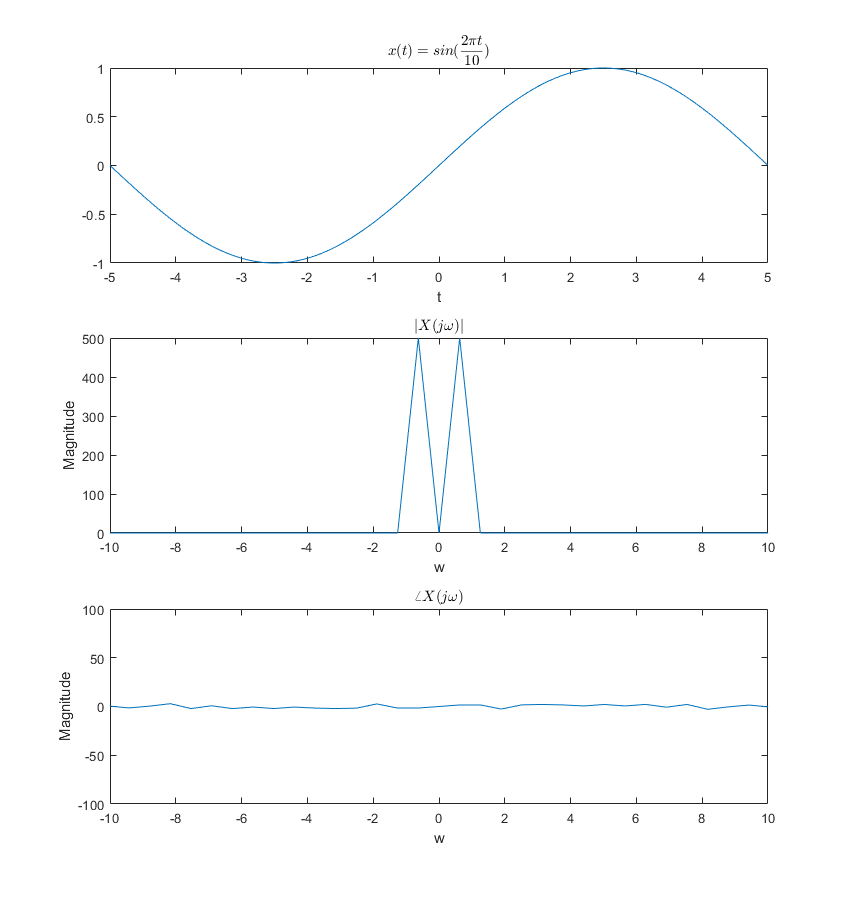
\includegraphics[width=\linewidth]{q2a}
\caption{$ = sin(\omega _{0}t)$}
\end{subfigure}
\begin{subfigure}[b]{.3\linewidth}
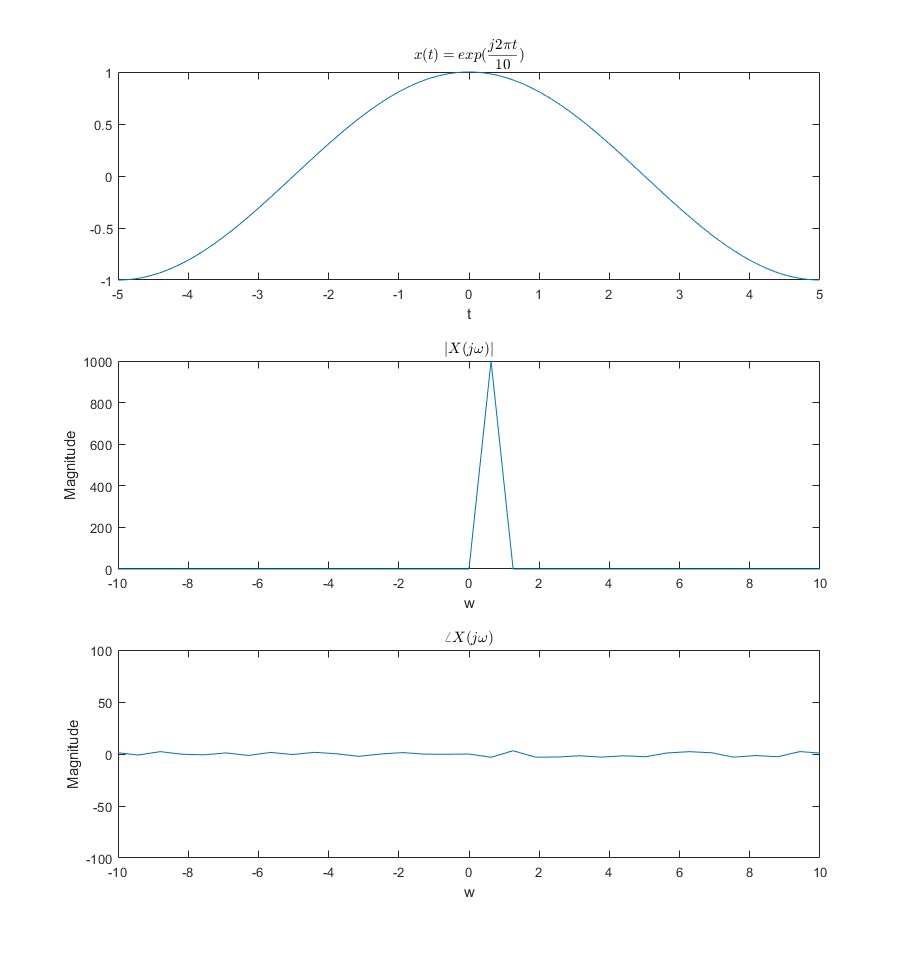
\includegraphics[width=\linewidth]{q2b}
\caption{$ = e^{j\omega _{0}t}$}
\end{subfigure}
\begin{subfigure}[b]{.3\linewidth}
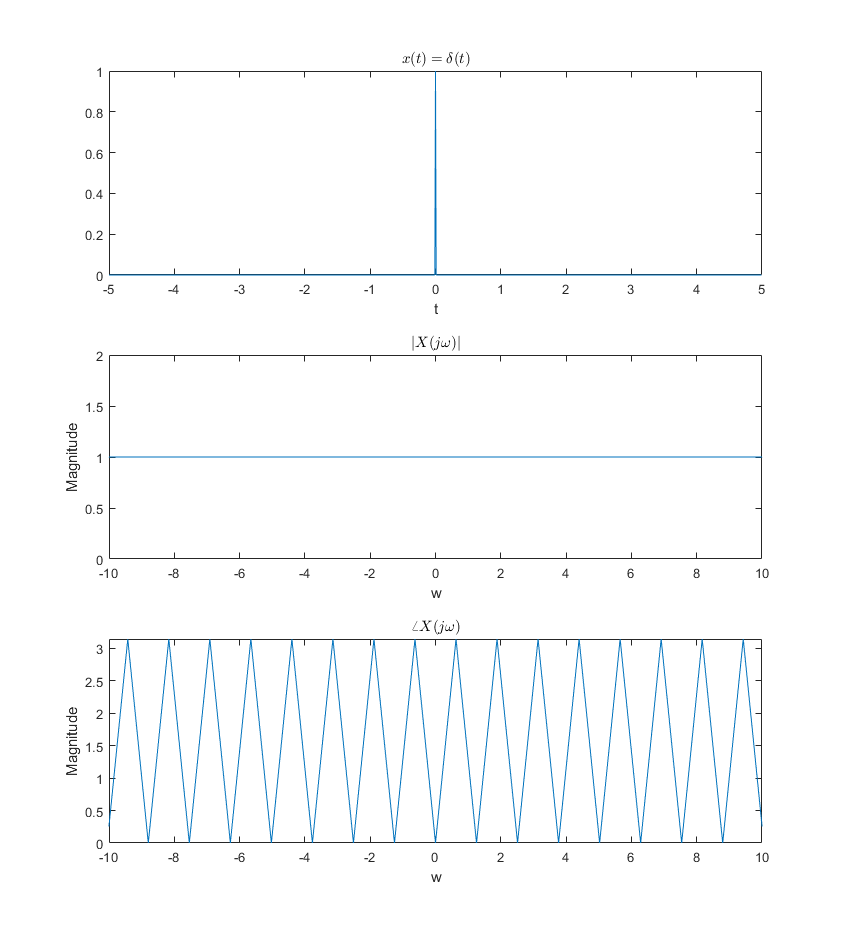
\includegraphics[width=\linewidth]{q2c}
\caption{$ = \delta (t)$}
\end{subfigure}

\begin{subfigure}[b]{.3\linewidth}
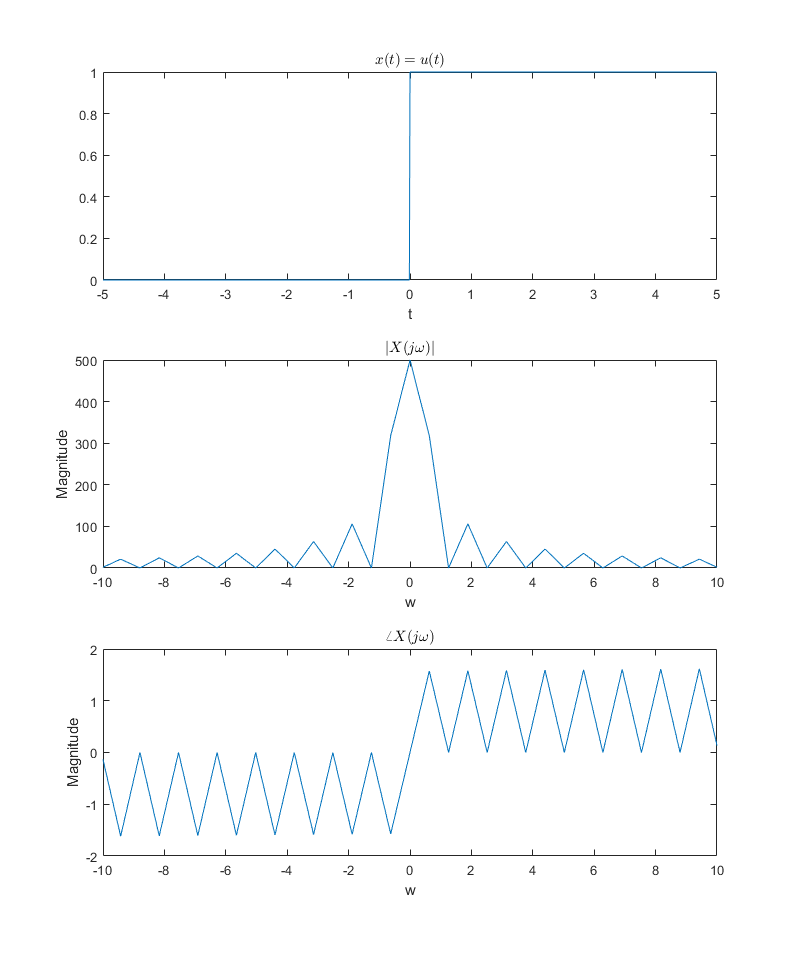
\includegraphics[width=\linewidth]{q2d}
\caption{$ = u(t)$}
\end{subfigure}
\begin{subfigure}[b]{.3\linewidth}
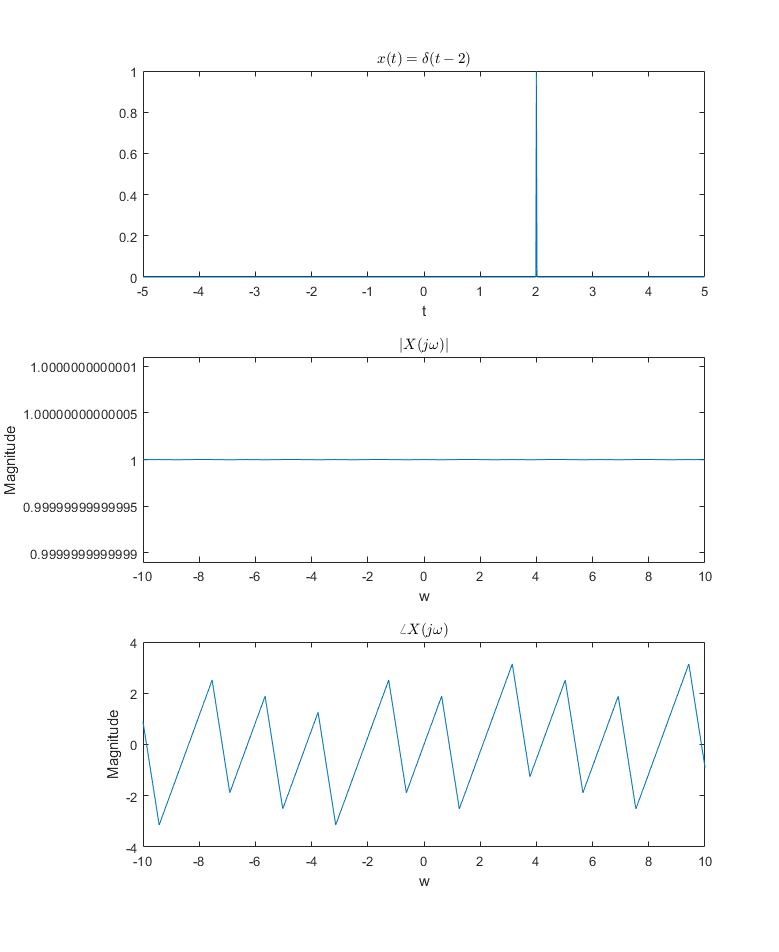
\includegraphics[width=\linewidth]{q2e}
\caption{$ = \delta (t-t_{0}) : t_{0}=2$}
\end{subfigure}
\begin{subfigure}[b]{.3\linewidth}
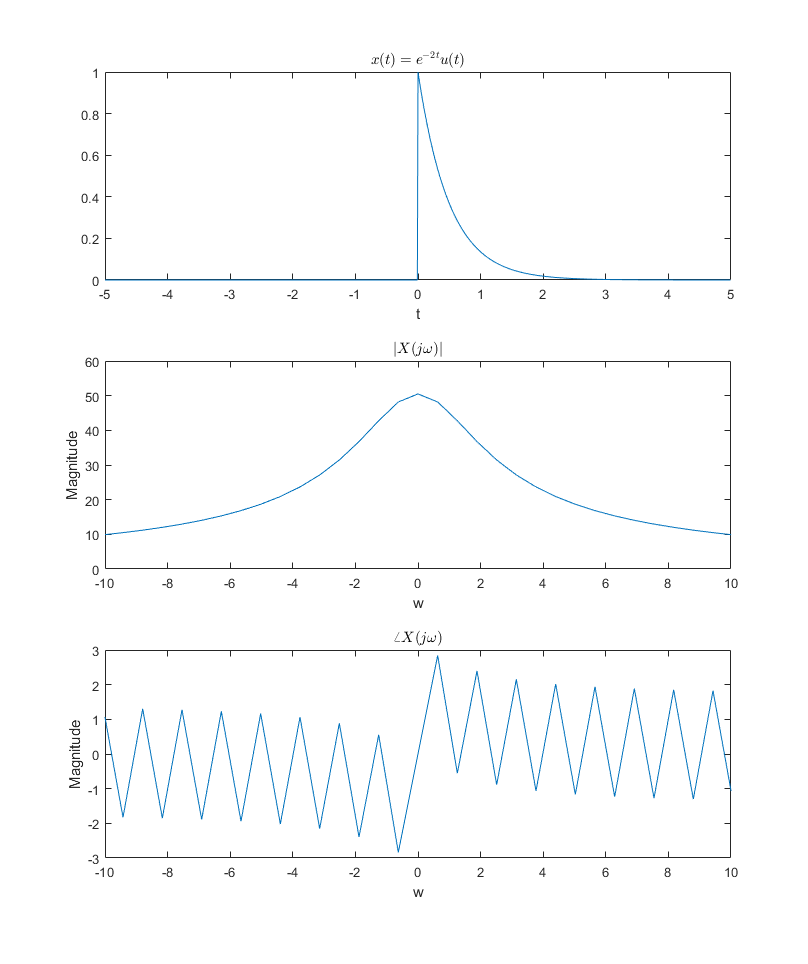
\includegraphics[width=\linewidth]{q2f}
\caption{$ = e^{-at}u(t) : a=2 $}
\end{subfigure}

\begin{subfigure}[b]{.3\linewidth}
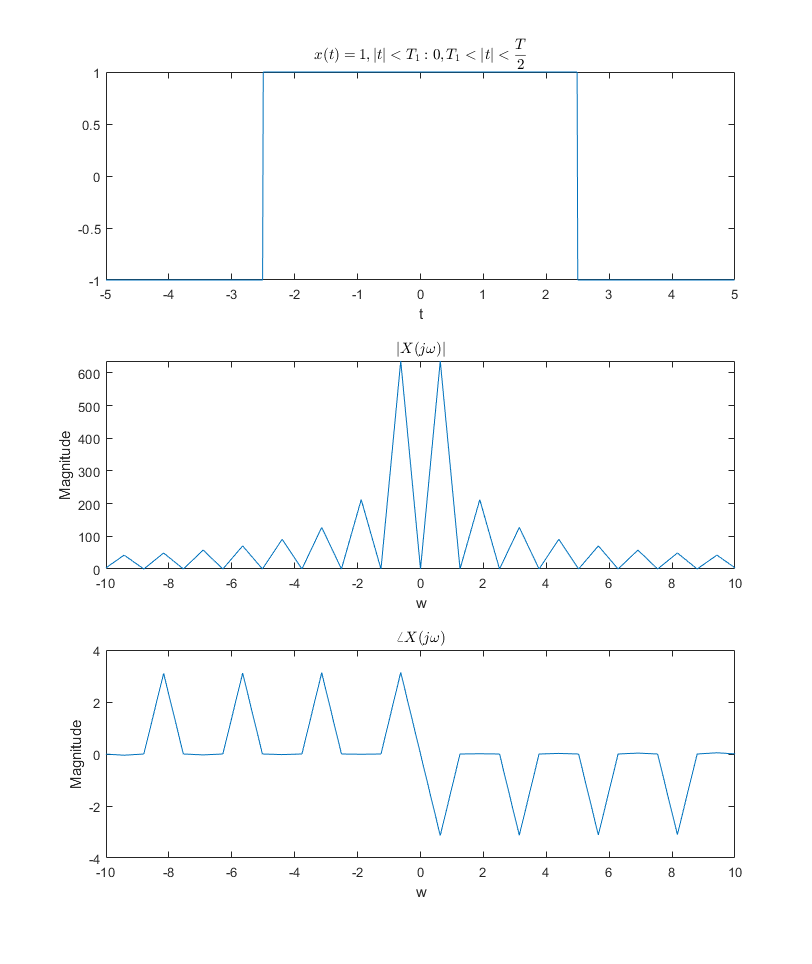
\includegraphics[width=\linewidth]{q2g}
\caption{ = \begin{cases}
			$1, & |t|<T_{1}$ \\
      		$0, & T_{1}<|t|< \frac{T}{2}$
   			\end{cases}}
\end{subfigure}
\caption{(2.a)}
\end{figure}

\newpage
\section{Other Fs's (Ref: Figure 2)}
\paragraph*{2.b)}
\begin{enumerate}
\item
$|X(j\omega)| = \delta (-\omega _{0} + \delta (\omega _{0})$
\item
$|X(j\omega)| = \delta (\omega _{0}$
\item
$|X(j\omega)| = 1$
\item
$|X(j\omega)| = \delta (0)$
\item
$|X(j\omega)| = 1$
\item
$|X(j\omega)| = |\dfrac{1}{j\omega + \alpha}|$
\item
$|X(j\omega)| = sinc(\omega)$

\end{enumerate}


\paragraph*{2.c)}
Anomalies in the phase of the first 2 are the same as previously discussed in 1.c, ie machine precision etc.
\subparagraph*{fig 2c}
The ideal Magnitude function for a zero centred delta is correctly plotted as a constant, but due to Matlab treating the delta as not perfectly zero centred the phase plot is not a constant, but instead in slightly modulated.
\subparagraph*{fig 2d}
The ideal Mag/Phase for the unit step should be a delta and a linear phase shift but as plotted in Matlab, it was treated as periodic, ie a squared pulse, so the plotted transform is that for a zero starting square pulse.
\subparagraph*{fig 2e}
The ideal Magnitude function for a shifted delta is correctly plotted as a constant, but due to Matlab treating the delta as not perfectly centred on its ideal. It should be a Sawtooth wave, which is a visible component but there is still some modulation.
\subparagraph*{fig 2f}
The magnitude is correctly plotted, but again the phase should be a smooth transition $\pm}$ 180 degrees, but Matlab plots oscillations of amplitude $\pi$.

\subparagraph*{fig 2e}
For this zero centred square phase correctly plots oscillations between 0 and $-\pi$ for $\omega > 0$ and oscillations between 0 and $+\pi$ for $\omega < 0$.
Although I am not sure abount the zero magnitude at $\omega$ = 0
%----------------------------------------------------------------------------------------
%	APPENDIX
%----------------------------------------------------------------------------------------
\newpage

\section{Appendix}

\subsection*{Figure 1:}
\lstinputlisting{q1.m}
\newpage
\subsection*{Figures 2:}
\lstinputlisting{q2.m}

\end{document}
